%%%%%
%
%	Добавить термоэлектронную эмиссию
%	Добавить электронный осциллограф
%	Флюоресценция
%
%%%%%%

\documentclass[14pt]{article}

\usepackage[utf8x]{inputenc}
\usepackage[russian]{babel}
\usepackage{graphicx}
\graphicspath{{images/}}
\DeclareGraphicsExtensions{.pdf,.png,.jpg}

\usepackage{amsmath}

\usepackage{geometry} % Меняем поля страницы
\geometry{left=2cm}% левое поле
\geometry{right=1.5cm}% правое поле
\geometry{top=2cm}% верхнее поле
\geometry{bottom=2cm}% нижнее поле

\renewcommand{\theenumi}{\arabic{enumi}}% Меняем везде перечисления на цифра.цифра
\renewcommand{\labelenumi}{\arabic{enumi}}% Меняем везде перечисления на цифра.цифра
\renewcommand{\theenumii}{.\arabic{enumii}}% Меняем везде перечисления на цифра.цифра
\renewcommand{\labelenumii}{\arabic{enumi}.\arabic{enumii}.}% Меняем везде перечисления на цифра.цифра
\renewcommand{\theenumiii}{.\arabic{enumiii}}% Меняем везде перечисления на цифра.цифра
\renewcommand{\labelenumiii}{\arabic{enumi}.\arabic{enumii}.\arabic{enumiii}.}% Меняем везде перечисления на цифра.цифра


\begin{document}

\begin{titlepage}
	\begin{center}
		\fontsize{18pt}{20pt}\selectfont
		\textbf{Работа 1.1.6.}	
	
		\vspace{5cm}
		\fontsize{24pt}{25pt}\selectfont
		Изучение электронного осциллографа
	\end{center}
	\begin{flushright}
		\fontsize{18pt}{20pt}\selectfont
		\vspace{14cm}
		\hspace{-3cm}
		\textit{Корнеев Е.С.}
	\end{flushright}		
\end{titlepage}

\newpage
\begin{center}
	\fontsize{16pt}{18pt}\selectfont	
	Изучение электронного осциллографа
\end{center}

\fontsize{14pt}{16pt}\selectfont
\vspace{1cm}
\textbf{Цель работы:} ознакомление с устройством и работой осциллографа и изучение его основных характеристик.

\vspace{0.5cm}
\textbf{В работе используются:} осциллограф, генераторы электрических сигналов, соединительные кабели.

\vspace{1cm}
Осциллограф --- регистрирующий прибор, в котором исследуемое напряжение (сигнал) преобразуется в видимый на экране график изменения напряжения во времени. Осциллограф широко используется в физическом эксперименте. С егоп помощью можно исследовать изменение во времени любых физических величин, которые могут быть преобразованы в электрические сигналы. 

Лабораторная работа проводится с использованием учебного осциллографа, разработанного на основе осциллографов С1-94 и С1-1. 

%%%%%
%
%	ЭЛЕКТРОННО-ЛУЧЕВАЯ ТРУБКА
%
%%%%%

\vspace{0.5cm}
\textbf{Электронно-лучевая трубка.} Основной частью электронного осциллографа, определяющей его важнейшие технические характеристики, является электронно-лучевая трубка (ЭЛТ). Трубка представляет собой стеклянную откачанную до высокого вакуума колбу, в которой расположены (рис. 1): подогреватель катода 1, катод 2, модулятор 3 (электрод, управляющий яркостью изображения), первый (фокусирующий) анод 4, второй (ускоряющий) анод 5, горизонтально и вертикально отклоняющие пластины 6 и 7, третий (ускоряющий) анод 8, экран 9.

\begin{figure}[h!]
	\center{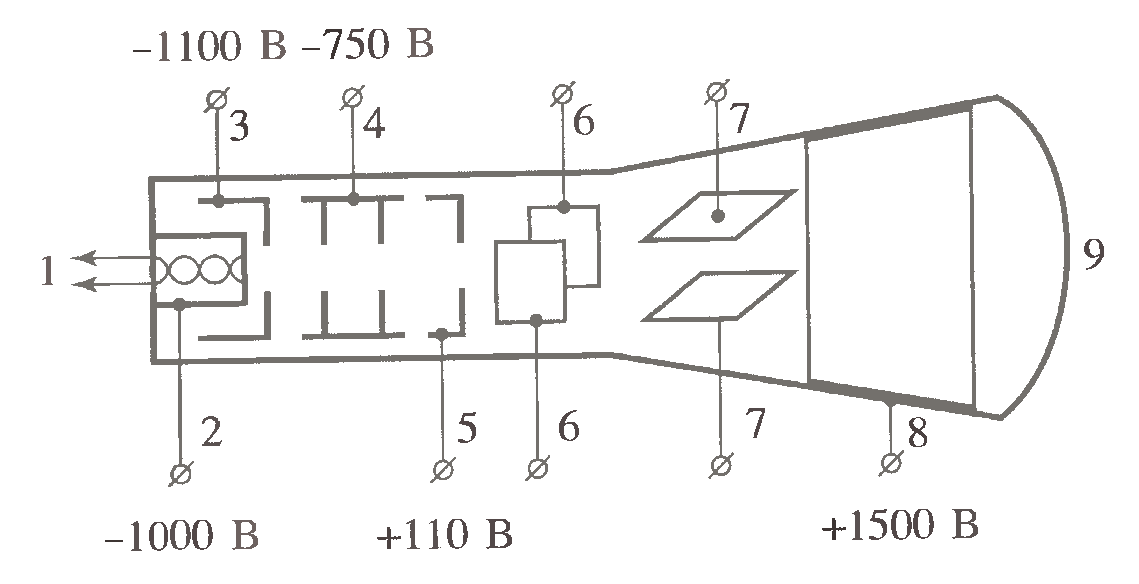
\includegraphics[width = 10cm]{1}}
	\caption{Электронно-лучевая трубка}
	\label{fig:image}
\end{figure}

Электронный пучок формируется системой электродов, называемых <<электронной пушкой>>: катод с нагревателем, модулятор, фокусирующий и ускоряющий аноды. Форма, размер, и расположение электродов подобраны таким образом, чтобы разгонять электроны и фокусировать пучок на экране. Потенциал первого (фокусирующего) анода относительно катода можно изменять ручкой <<ФОКУС>>. Размер пятна на экране в значительной степени определяется качеством фокусирующей системы, его диаметр обычно не превышает 1мм. Яркость пятна на экране осциллографа определяется током электронного луча, который может регулироваться изменением напряжения на модуляторе ручкой <<ЯРКОСТЬ>>. Экраном осциллографа является покрытая флюоресцирующим веществом стенка трубки, на которую попадает электронный пучок.

На пути к экрану сформированный пучок электронов проходит две пары отклоняющих пластин. Две вертикально расположенные пластины образуют плоский конденсатор, электрическое поле которого способно отклонять пучок в горизонтальном направлении (горизонтально отклоняющие пластины). Аналогично поле горизонтально расположенных пластин вызывает вертикальное отклонение пучка (вертикально отклоняющие пластины). Подавая на пластины соответствующие напряжения, можно <<нарисовать>> электронным лучом на экране некоторую фигуру. 

\begin{figure}[h!]
	\center{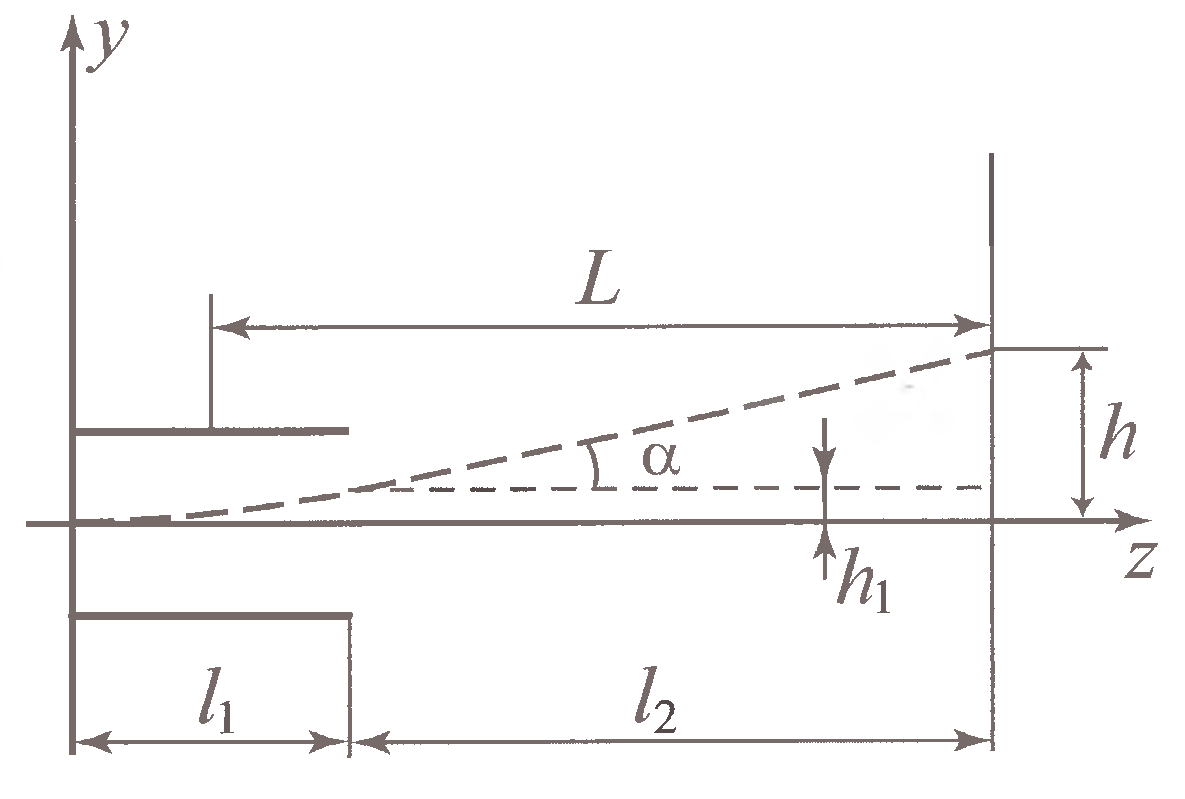
\includegraphics[width = 10cm]{2}}
	\caption{Отклонение луча в электрическом поле пластин}
	\label{fig:image}
\end{figure}

Рассмотрим движение электронов в электрическом поле отклоняющих пластин (рис. 2). Пусть электрон со скоростью $v_0$ влетает в однородное электрическое поле пары пластин и движется вдоль оси $z$, т.е. перпендикулярно к линиям напряженности электрического поля. Движение электрона вдоль оси $z$ является равномерным, а вдоль оси $y$ --- равноускоренным:

\begin{equation}
z = v_0t,~
y = \frac{at^2}{2}
\end{equation}

Ускорение можно найти с помощью второго закона Ньютона:

\begin{equation}
a = \frac{eE_y}{m}
\end{equation}

\noindent Из (1) и (2) найдем:

\begin{equation}
y = \frac{eE_y}{2mv_0^2}z^2
\end{equation}

\noindent Как следует из (3), траектория электрона между отклоняющими пластинами представляет собой параболу. На выходе из пластин электрон отклоняется от первоначального направления на расстояние $h_1$ и летит под углом $\alpha$ к оси $z$:

\begin{equation}
h_1 = \frac{eE_y}{2mv_0^2}l_1^2,~ \tg \alpha = \frac{eE_y}{mv_0^2}l_1
\end{equation}

\noindent где $l_1$ - длина пластин. Выйдя из пластин, электрон движется по прямой. Смещение $h$ электронного пятна на экране осциллографа получим из рис. 2:

\begin{equation}
h = h_1 + l_2\tg \alpha = \frac{eE_yl_1}{mv_0^2}\left(\frac{l_1}{2}+l_2\right)
\end{equation}

Обозначим расстояние от середины пластин до экрана через $L$. Тогда

\begin{equation}
h =  \frac{eE_yl_1L}{mv_0^2}
\end{equation}

Скорость $v_0$, которую имеют электроны, проходящие между пластинами, определяется ускоряющим напряжением $U_a$ на втором аноде:

\begin{equation}
\frac{mv_0^2}{2} = eU_a
\end{equation}

Напряженность $E_y$ электрического поля между отклоняющими пластинами 

\begin{equation}
E_y = \frac{U_y}{d}
\end{equation}

\noindent где $U_y$ --- разность потенциалов между пластинами, а $d$ --- расстояние между ними. Окончательно из (6) --- (8) получим

\begin{equation}
h = \frac{l_1L}{2dU_a}U_y
\end{equation}

\noindent Таким образом, смещение луча пропорционально отклоняющему напряжению $U_y$. Коэффициент пропорциональности в (9) называется чувствительность $k$ трубки к напряжению:

\begin{equation}
k = \frac{h}{U_y} = \frac{l_1L}{2dU_a}\left[\frac{\text{см}}{\text{В}}\right]
\end{equation}

\noindent Аналогично вычисляется чувствительность трубки к напряжению на второй паре пластин. 

Формула (9) применима и в том случае, когда на отклоняющие пластины подается переменное напряжение, но при условии, что оно мало изменяется за время $\tau$ пролета электрона между пастинами. Характерными интервалами времени $T$, которое определяет скорость изменения переменного сигнала, могут быть: период сигнала, длительность импульса, время нарастания сигнала до некоторого уровня и т.д. Оценим минимальное значение $T_{min}$ времени $T$, при котором выполняется условие: $T_{min} \ll \tau$. Скорость электронов после вылета из <<электронной пушки>> составляет примерно $2*10^{-7}$ м/с (при $U_a \approx 10^3$ В). Полагая $l = 3$ см, для времени пролета $\tau$ получим: $\tau = 1.5*10^{-9}$ с. Тогда, выбирая условие $T_{min}/\tau \ge 10$ в качестве критерия применимости формулы (9) для переменного сигнала, имеем $T_{min} = 15*10^{-9}$ с. Таким образом, выражение (9) будет определять точки попадания электрона на экран ЭЛТ, если частота синусоидального сигнала, подаваемого на отклоняющие пластины, не превышает $\sim 10^8 \text{Гц} = 0.1 \text{ГГц}$. 

На практике, однако, максимальная частота оказывается существенно меньше. Чувствительность трубки к напряжению составляет доли мм/В, поэтому исследуемый сигнал, подаваемый на отклоняющие пластины, приходится предварительно усиливать. Всякий усилитель арактеризуется диапазоном частот, в пределах которого его коэффициент практически не меняется, а вне этого диапазона резко падает. Граничная (максимальная) частота усилителя определяется постоянной времени электрической схемы осциллографа. Как правило, рабочий диапазон частот осциллографа ограничивается именно рабочим диапазоном частот усилителя, на который подается исследуемый сигнал. 

Таким образом, в рабочем диапазоне  частот осциллографа (для учебного осциллографа 0-1 МГц) смещение луча по вертикали (или горизонтали) на экране ЭЛТ можно считать пропорциональным мгновенному значению напряжения на соответствующих отклоняющих пластинах.

%%%%%%%%%%%%%%%%%%%%%%%%%%%%%%
%
%	РАЗВЕРТКА
%
%%%%%%%%%%%%%%%%%%%%%%%%%%%%%%

\vspace{0.5cm}
\textbf{Развертка.} Из формулы (9) следует, что координаты $x$ и $y$ точки попадания электронного луча на ЭЛТ (относительно ее центра) пропорциональны мгновенным значениям напряжений $U_x(t)$  и $U_y(t)$, подаваемых на горизонтально и вертикально отклоняющие пластины.

Так как величина исследуемых сигналов лежит в достаточно широком диапазоне (от десятка микровольт до сотен вольт), а чувствительность отклоняющих пластин ЭЛТ по напряжению сравнительно невелика (доли мм/В), то в зависимости от величины подаваемого на вход сигнала его необходимо усиливать или, в случае большого сигнала, предварительно ослаблять.

Для усиления слабых сигналов в осциллографе имеются усилители вертикального отклонения луча (усилитель <<Y>>) и горизонтального ---  усилитель <<X>>. На входе усилителя <<Y>> установлен аттенюатор (делитель), позволяющий ослаблять входной сигнал в заданное число раз.

Для получения на экране ЭЛТ <<изображения>> периодического электрического сигнала $U_c(t)$ необходимо выполнение двух условий:

1. Подаваемое на вертикально отклоняющие пластины напряжение $U_y$ должно линейно зависеть от самого сигнала $U_c$:

\begin{equation}
U_y(t) = U_{0y} + k_{yu}U_c(t)
\end{equation}

\noindent Здесь $U_{0y}$ --- постоянное напряжение, определяющее расположение графика сигнала по оси $Y$ на экране ЭЛТ, $k_{yu}$ — коэффициент преобразования входного сигнала каналом вертикального отклонения.

2. Подаваемое на горизонтально отклоняющие пластины напряжение $U_x$ должно линейно зависеть от времени $t$:

\begin{equation}
U_x = U_{0x} + k_{xu}(t)
\end{equation}

\noindent Здесь $U_{0x}$ — постоянное напряжение, определяющее расположение графика сигнала по оси Х на экране ЭЛТ, $k_{xu}$ — коэффициент пропорциональности, зависящий от рабочих характеристик генератора развертки и усилителя <<X>>.

\begin{figure}[h!]
	\center{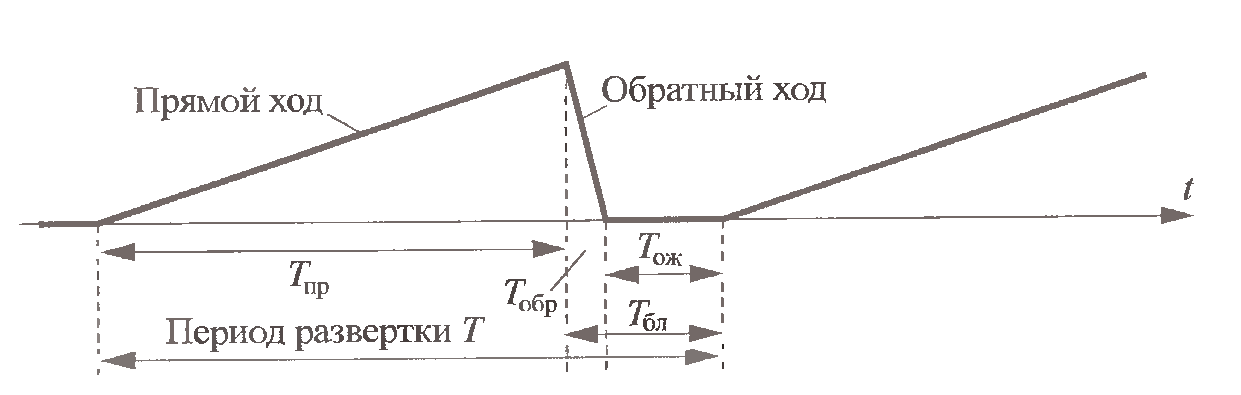
\includegraphics[width = 12cm]{3}}
	\caption{Напряжение развертки}
	\label{fig:image}
\end{figure}

Напряжение пилообразной формы, которое вырабатывает генератор развертки осциллографа, называемое также напряжением развертки, изображено на рис.~3. B течение прямого хода луча ($T_{\text{пр}}$) напряжение изменяется до максимального значения так, что луч с постоянной скоростью проходит весь экран слева направо. После завершения прямого хода луча начинается процесс обратного хода луча 
($T_{\text{обр}}$), когда напряжение развертки возвращается к первоначальному уровню, и луч переходит в исходное положение в левый край экрана. Скорость изменения напряжения прямого хода развертки, т. е. масштаб по оси $X$, задается расположенным на передней панели осциллографа переключателем «ВРЕМЯ/ДЕЛ», проградуированным во времени, за которое луч проходит одно большое деление сетки экрана. Наличие интервала ожидания $T_{\text{ож}}$ позволяет изменять масштаб по оси $X$ независимо от периода развертки.

Во время <<прямого>> хода пилы на модулятор <<электронной пушки>> подается положительное относительно катода напряжение, при этом на экране виден светящийся след электронного луча. Во время <<обратного>> хода пилы (т.е. на интервале блокировки $T_{\text{бл}}$) напряжение на модуляторе <<запирает>> трубку. В результате электронный луч на интервале блокировки не вызывает свечения экрана.

%%%%%%%%%%%%%%%%%%%%%%%%%%%%%%%%
%
%	СИНХРОНИЗАЦИЯ
%
%%%%%%%%%%%%%%%%%%%%%%%%%%%%%%%%

\vspace{0.5cm}
\textbf{Синхронизация.} При наблюдении периодических и особенно быстропротекающих процессов важно получить на экране осциллографа неподвижное изображение сигнала. Для этого нужно, чтобы период развертки был кратен периоду изучаемого сигнала. Однако, как правило, точное соотношение периодов соблюсти трудно из-за нестабильности генератора развертки или самого изучаемого процесса. Поэтому используют принудительное согласование периодов, при котором изучаемое напряжение <<навязывает>> свой период генератору развертки. При этом начало прямого хода развертки должно совпадать строго с одной и той же характерной точкой исследуемого периодического сигнала. Процесс привязки начала развертки к характерным точкам сигнала называется синхронизацией развертки с сигналом. Этот способ синхронизации поясняется осциллограммами, изображенными на рис. 4.

\begin{figure}[h!]
	\center{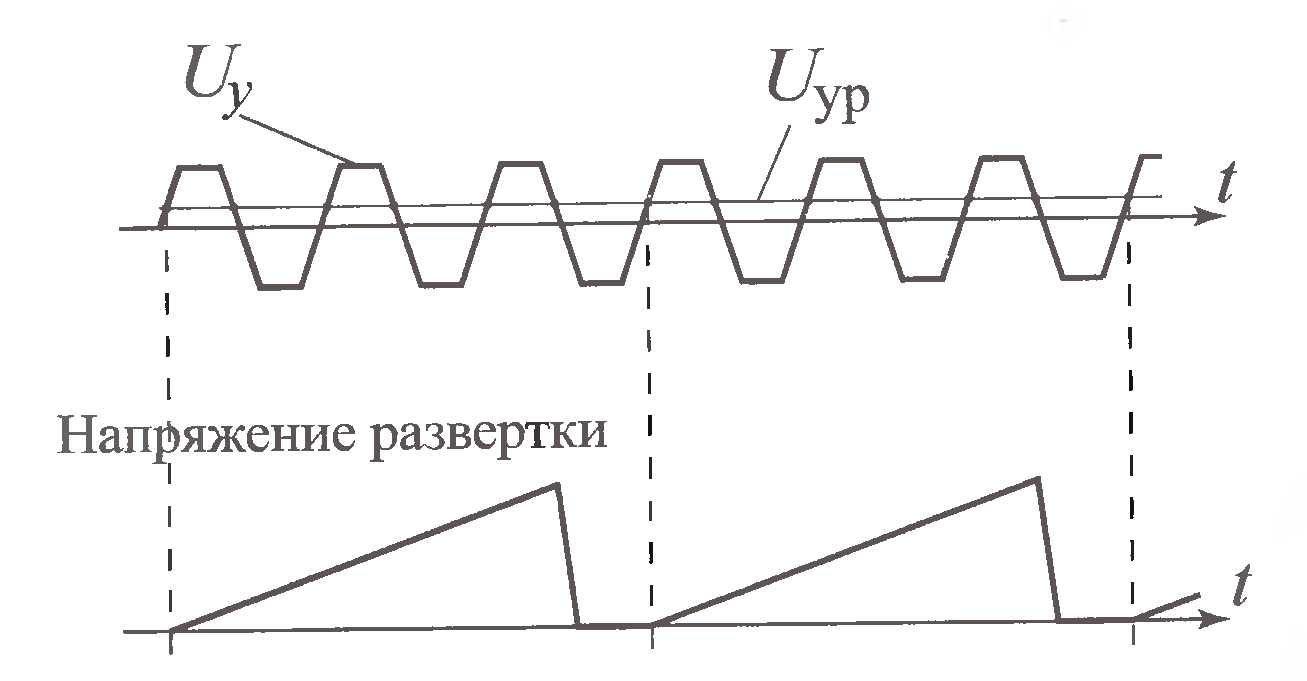
\includegraphics[width = 10cm]{4}}
	\caption{Процесс синхронизации генератора развертки}
	\label{fig:image}
\end{figure}

Сигнал произвольной формы $U_y$ (на рисунке — сигнал трапециевидной формы) сравнивается с пороговым напряжением $U_{\text{ур}}$ (уровнем синхронизации), устанавливаемым ручкой <<УРОВЕНЬ>>. В момент пересечения сигналом $U_y$ уровня $U_{\text{ур}}$ снизу вверх запускается прямой ход развертки (<<пила>>), при условии, что это произошло на интервале ожидания $T_{\text{ож}}$ (рис. 3 и 4). Запуск <<пилы>> может производиться при пересечении сигнала $U_y$ уровня $U_{\text{ур}}$ как снизу вверх (как на рис. 4), так и сверху вниз в зависимости от выбранного положения переключателя режимов синхронизации развертки на передней панели осциллографа (<<ЗАПУСК~+>> или <<ЗАПУСК~--->>). Напряжение $U_{\text{ур}}$ изменяется при вращении ручки «УРОВЕНЬ» на передней панели осциллографа, что позволяет совместно с переключателем <<ЗАПУСК~+,~--->> выбрать фазу сигнала в начале развертки, исходя из наилучшей устойчивости синхронизации и удобства наблюдения. Если $U_{\text{ур}}$ не пересекает $U_y$, то синхронизация невозможна.

Генератор развертки может работать в автоматическом или ждущем режимах, выбираемых тумблером <<АВТ/ЖДУЩ>>. В автоматическом режиме время ожидания $T_{\text{ож}}$ не может быть больше некоторого максимального времени ожидания $T_{\text{ож, max}}$. Если на максимальном интервале ожидания не произошло пересечения $U_y$ и $U_{\text{ур}}$, то происходит автоматический запуск прямого хода развертки в момент, не связанный с определенной фазой исследуемого сигнала, а пилообразный сигнал будет иметь период $T_{\text{п, авт}}$ , определяемый только внутренними параметрами осциллографа. В этом случае изображение исследуемого сигнала на экране перемещается влево или вправо (<<бежит>>), а при отсутствии исследуемого сигнала видна горизонтальная линиия развертки.

При пересечении $U_y$ и $U_{\text{ур}}$ на интервале ожидания происходит запуск прямого хода развертки в момент, связанный с определенной фазой исследуемого сигнала. На экране при этом наблюдается неподвижное изображение сигнала.

Синхронизация в автоматическом режиме возможна лишь в случае, когда собственный период генератора развертки больше периода исследуемого сигнала $T_{\text{п, авт}}>T_c$. B противном случае за первым циклом запуска сигнала развертки будет следовать один или несколько автоматических запусков прямого хода <<пилы>> в моменты времени, не привязанные к определенной фазе исследуемого сигнала, т.е. произойдет наложение друг на друга различных изображений сигнала.

В ждущем режиме запуск прямого хода развертки происходит только при наличии пересечения $U_y$ и $U_{\text{ур}}$ на интервале ожидания $T_{\text{ож}}$, причем интервал ожидания $T_{\text{ож}}$ в этом режиме может быть сколь угодно большим, а синхронизация осуществляется при любом периоде исследуемого сигнала $U_c(t)$. Наблюдение на экране малой части периода процесса (например, фронта импульса или короткого импульса, длительность которого много меньше периода следования импульсов) возможно только в ждущем режиме.

Кроме синхронизации развертки исследуемым сигналом, предусмотрен режим синхронизации внешним сигналом (вместо $U_y$), синхронным по отношению к исследуемому сигналу. Этот сигнал полается на гнездо <<ВНЕШ. ЗАП>> на передней панели осциллографа. Переключатель <<ЗАПУСК>> при этом должен находиться в положении <<ВНЕШ>>. Работа элементов схемы синхронизации и развертки в этом случае аналогична описанной выше.

Выбор диапазона (масштаба) развертки осуществляется переключателем <<ВРЕМЯ/ДЕЛ>>.

Удобный для наблюдения на экране размер изображения по вертикали устанавливается переключателем <<V/ДЕЛ>>, проградуированным в величине напряжения, приводящего к перемещению луча по вертикали на одно большое деление (эта величина называется коэффициентом отклонения). Для смещения изображения по вертикали предусмотрен потенциометр «$\updownarrow$», который изменяет постоянную составляющую $U_{0y}$ (см. формулу (11)).

В процессе работы с осциллографом всегда следует учитывать характеристики каналов вертикального и горизонтального отклонения: амплитудно-частотную характеристику (АЧХ) и фазово-частотную характеристику (ФЧХ). Если на вход <<Y>> осциллографа подается синусоидальное напряжение $U_y = U_0\sin (2\pi ft)$ амплитудой $U_0$ и частотой $f$, то для перемещения луча на экране ЭЛТ можно записать: $y = y_0(f)\sin (2\pi ft + \Delta \Phi_y(f))$. Здесь $y_0(f)$ --- амплитуда перемещения луча на частоте $f$, $\Delta \Phi_y(f)$ --- разность между фазой колебаний перемещения луча $y$ и фазой колебаний входного сигнала $U_y$ на частоте $f$ (сдвиг фаз).

Тогда АЧХ канала вертикального отклонения есть зависимость

$$K_y(f) = \frac{y_0(f)}{U_0}$$

\noindent а ФЧХ - зависимость $\Delta \Phi_y(f)$. АЧХ и ФЧХ канала горизонтального отклонения определяются аналогично.

Как правило, АЧХ $K_y(f)$ остается практически постоянной $K_y = K_{y, max}$ в диапазоне частот от $f_{min}$ до $f_{max}$ и уменьшается на частотах  $f < f_{min}$ и $f > f_{max}$. Диапазон частот от $f_{min}$ до $f_{max}$ называется полосой пропускания. Значения частот $f_{min}$ и $f_{max}$ определяют из условий

$$\frac{K_y(f_{min})}{K_{y, min}} = \frac{K_y(f_{max})}{K_{y, max}} = \frac{1}{\sqrt{2}} \approx 0.7$$

Непостоянство характеристик $K_y(f)$ и $\Delta \Phi(f)$ во всем диапазоне частот прводит‚ например, к искажению формы импульсного сигнала высокой частоты при его преобразовании в канале вертикального отклонения осциллографа.

Канал <<Y>> может быть использован с открытым или закрытым входом. В первом случае передается как переменная $U_\sim$, так и постоянная $U_=$ составляющие сигнала, во втором — только переменная. При работе в режиме с закрытым входом постоянная составляющая сигнала задерживается включенным на входе разделительным конденсатором.
Путем переключения тумблера <<$\sim/\simeq$>> на передней панели осциллографа можно выбрать необходимый ВХОД усилителя <<Y>>. Канал горизонтального отклонения имеет аналогичный усилитель <<X>>.
При наблюдении зависимости  $U_y = F(U_x)$ сигнал $U_x$ подается на закрытый вход <<$\rightarrow \supset X$>>. В учебном осциллографе размер изображения по горизонтали не регулируется. Для смещения изображения по горизонатали предусмотрен потенциометр <<$\leftrightarrow$>>, изменяющий постоянную составляющую $U_{0x}$ (см. формулу (12)).

%%%%%%%%%%%%%%%%%%%%%%%%%%%%%%%
%
%	ЛИССАЖУ
%
%%%%%%%%%%%%%%%%%%%%%%%%%%%%%%%

\vspace{0.5cm}
\textbf{Фигуры Лиссажу.} При сложении двух взаимно перпендикулярных колебаний с равными или кратными частотами, поданных на входы осциллографа, луч описывает на экране неподвижные замкнутые кривые, которые называются кривыми Лиссажу. При небольшом нарушении кратности частот форма фигур медленно меняется, а при большом --- картина размывается.

Пусть на горизонтально отклоняющие пластины ЭЛТ подается сигнал $U_x = U_a\cos (2\pi ft + \varphi_1)$ (при этом собственный генератор развертки осциллографа должен быть, конечно, выключен), а на вертикально отклоняющие пластины поступает смещенный по фазе сигнал той же частоты $U_y = U_b\cos (2\pi ft + \varphi_2), \varphi_1 \ne \varphi_2$.

При чувствительностях пластин $k_x$ и $k_y$ координаты $x$, $y$ светящегося пятна на экране будут определяться выражениями

$$x = A\cos (2\pi ft + \varphi_1)$$

$$y = B\cos (2\pi ft + \varphi_2)$$

$$A = k_xU_a$$

$$B = k_yU_b$$

Исключив из этих уравнений время $t$, нетрудно получить уравнение траектории движения луча:

$$\frac{x^2}{A^2} + \frac{y^2}{B^2} - 2\frac{xy}{AB}\cos (\varphi_2 - \varphi_1) = 
  \sin^2 (\varphi_2 - \varphi_1)$$

Таким образом, фигура, которую описывает луч при сложении колебаний, имеющих одинаковую частоту, представляет собой эллипс. Ориентация этого эллипса зависит от разности фаз колебаний $(\varphi_2 - \varphi_1)$

В общем случае вид фигуры Лиссажу зависит от соотношений между периодами (частотами), фазами, и амплитудами слкладываемых колебаний. Некоторые частные случаи фигур Лиссажу для разных периодов и фаз показаны на рис. 5. Зная параметры одного колебания, например, $f_x$, можно по фигуре Лиссажу определить параметры другого колебания --- $f_y$. На полученное изображение накладывают мысленно две линии --- горизонтальную и вертикальную, не проходящие через узлы фигуры. Фиксируют число пересечений с горизонтальной линией $n_x$ и вертикальной $n_y$, тогда отношение частот $f_y/f_x = n_x/n_y$.

Если одно или оба колебания происходят не по гармоническому, а по более сложному закону, то получаются траектории более сложной формы. 

\begin{figure}[h!]
	\center{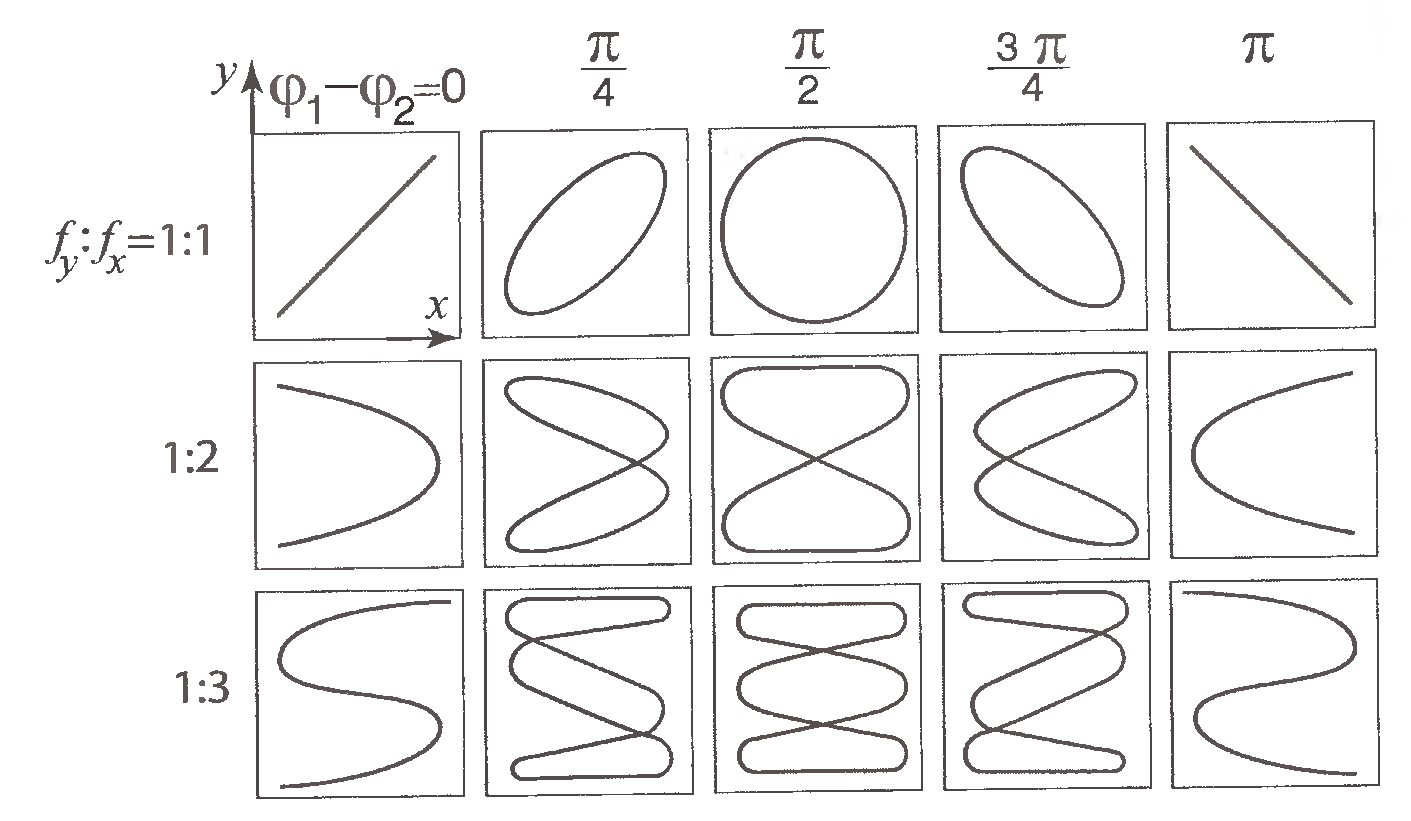
\includegraphics[width = 10cm]{5}}
	\caption{Фигуры Лиссажу для колебаний одинаковой амплитуды}
	\label{fig:image}
\end{figure}

%%%%%%%%%%%%%%%%%%%%%%%%%%%%%%%%
%
%	КАЛИБРАТОР
%
%%%%%%%%%%%%%%%%%%%%%%%%%%%%%%%%

\vspace{0.5cm}
\textbf{Калибратор.} Для проверки коэффициентов отклонения и развертки в осциллографе формируется внутренний калибровочный сигнал --- прямоугольные импульсы напряжения с частотой повторения 50 Гц и фиксированной амплитудой. При поступлении этих импульсов на вход <<Y>> (переключатель <<V/ДЕЛ>> --- в положении К) отклонение луча по оси $Y$ должно составлять 4.5-5.0 делений, а период колебаний - 20 мс по оси $X$.

%%%%%%%%%%%%%%%%%%%%%%%%%%%%%%%
%
%	ИЗМЕРЕНИЯ
%
%%%%%%%%%%%%%%%%%%%%%%%%%%%%%%%

\vspace{1cm}
\textbf{Приступаем к работе}

\vspace{0.5cm}
1. \textbf{Наблюдение периодического сигнала от генератора и измерение его частоты.} 

Получим на экране осциллографа устойчивую картину периодического (синусоидального) сигнала, подаваемого с генератора, и с помощью горизонтальной шкалы экрана осциллографа проведем измерение периода и частоты сигнала.

Измерим период наблюдаемого сигнала $T$ и рассчитайте его частоту $f$. Оцените погрешность измерения периода $\Delta T$ и частоты $\Delta f$ с помощью осциллографа.

Повторим измерения для 3—5 частот из всего диапазона работы звукового генератора. Результаты занесем в таблицу.

%%%%%
%
%	ТАБЛИЦА 1
%
%%%%%

\vspace{0.5cm}
2. \textbf{Измерение амплитуды сигнала.} 

С помощью вертикальной шкалы экрана осциллографа измерим отношение максимальной и минимальной амплитуд напряжений $U_{max}/U_min$, которые способен выдавать генератор. Измерения проведем на частоте $f = 1$ кГц.

Выразим отношение максимального и минимального уровней сигнала $\beta_{21}$ в децибелах [дБ]. Определим по формуле:

$$\beta_{21} = 10 \ln\left(\frac{P_2}{P_1}\right) = 20 \ln\left(\frac{U_2}{U_1}\right)$$

где $P_2/P_1$ — отношение средних мощностей, $U_2/U_1$ — отношение амплитуд некоторых двух сигналов (здесь учтено, что мощность пропорциональна квадрату амплитуды $P \propto U^2$).

%%%%%
%
%	ТАБЛИЦА 2 - beta, U1, U2
%
%%%%%

\vspace{0.5cm}
3. \textbf{Измерение амплитудно-частотной характеристики осциллографа.} 

Проведем измерение АЧХ используемого в работе осциллографа во всём диапазоне рабочих частот генератора. Для этого установим частоту сигнала генератора $f = 1$ кГц и получим устойчивое изображение синусоиды на экране. Установим амплитуду генератора, близкую к максимальной и подберем масштаб вертикальной шкалы осциллографа так, чтобы размах сигнала на экране составил $2U_0 = 6$ дел. Далее при измерениях по данному пункту амплитуда сигнала на генераторе $U_0$ будет оставаться неизменной. Изменяя частоту $f$ звукового генератора во всем доступном диапазоне исследуем зависимость отношения амплитуды сигнала на осциллографе $U(f)$ к исходной $U_0$ в зависимости от частоты:

$$K(f) = \frac{U(f)}{U_0}$$

В области частот, где $K$ отличается от единицы, проведем подробные измерения $K(f)$. Измерения АЧХ $K(f)$ проведем для одного из каналов осциллографа при открытом $(DC, \simeq)$ и при закрытом $(AC, \sim)$ входе. Результаты занесем в таблицу.

%%%%%
%
%	ТАБЛИЦА 3 
%
%%%%%

%%%%%
%
%	ГРАФИКИ
%
%%%%%

\vspace{0.5cm}
4. \textbf{Изучение влияния АЧХ на искажение сигнала.}

Установим на генераторе прямоугольные импульсы, получим на экране устойчивую картину прямоугольных импульсов на частоте $f = 1$ кГц. Изменяя частоту генератора во всём диапазоне, пронаблюдаем, как меняется вид отображаемого на осциллографе сигнала для открытого и закрытого входов. Зарисуем характерный вид полученных осциллограмм для частот $f$, при которых форма прямоугольных импульсов существенно искажается. 

%%%%%
%
%	ОБЪЯСНЕНИЕ
%
%%%%%

\vspace{0.5cm}
5. \textbf{Измерение разности фазово-частотных характеристик каналов осциллографа.}

Осциллограф может быть использован для измерения разности фаз между подаваемыми на него сигналами, при этом однако необходимо учитывать, что каналы X и Y могут иметь разные ФЧХ. Проведем измерения разности фаз, возникающей при подаче одного и того же сигнала на разные каналы осциллографа, в зависимости от частоты сигнала.

Подадим напряжение $f = 1$ КГц на входы осциллографа и включим развертку $X-Y$. В этом режиме отклонение луча на экране пропорционально подаваемым на каналы напряжениям $Y(t) = k_yU_y(t)$, $X	(t) = k_xU_x(t)$. Выключим каналы и установим точку в центр экрана, затем получим изображение отрезка, наклоненного под углом $45^{\circ}$. Изменяя частоту генератора $f$ во всем доступном диапазоне, найдем участки, на которых изображение на экране переходит из отрезка в невырожденный эллипс (рис. 6). На этих участках проведем подробное измерение разности фаз $\Delta \varphi(t)$ между каналами $X$ и $Y$ в зависимости от частоты.

\begin{figure}[h!]
	\center{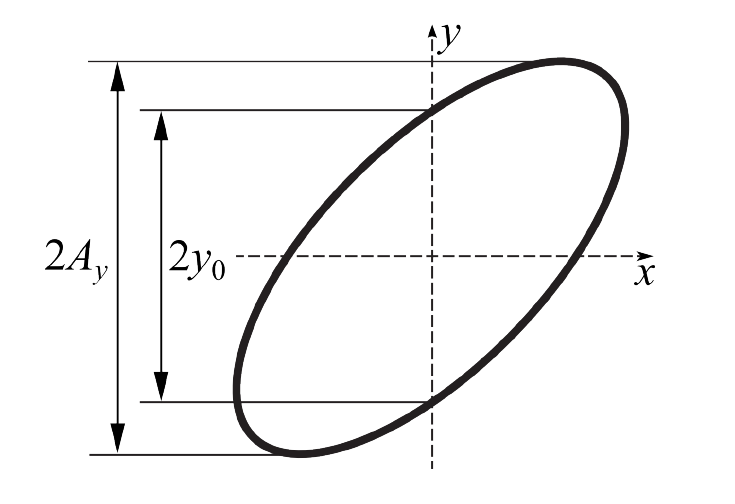
\includegraphics[width = 8cm]{6_2}}
	\caption{Разность фаз сигналов}
	\label{fig:image}
\end{figure}

При подаче на взаимно перпендикулярные отклоняющие пластины двух синусоидальных сигналов траектория луча на экране осциллографа представляет собой эллипс и может быть в общем виде описана уравнениями

\setcounter{equation}{0}
\begin{equation}
x(t) = A_x \sin(\omega t + \varphi_x),~
y(t) = A_y \sin(\omega t + \varphi_y)
\end{equation}

\noindent Разность фаз $\Delta\varphi = \varphi_y - \varphi_x$ можно выразить, например, положив в (1) $\omega t = - \Delta x$, после чего нетрудно получить

\begin{equation}
\Delta \left|\varphi\right| = \left|\frac{y_0}{A_y}\right|
\end{equation}

\noindent где $y_0$ --- отклонение луча по вертикали в тот момент, когда его абсцисса равна 0; $A_y$ --- амплитуда колебаний по оси 
$y$ (рис. 6). Тогда возможные значения разности фаз:

\begin{equation}
\left|\Delta \varphi\right| = \arcsin \left|\frac{y_0}{A_y}\right|
\end{equation}

\noindent или

\begin{equation}
\left|\Delta \varphi\right| = \pi - \arcsin \left|\frac{y_0}{A_y}\right|
\end{equation}

\noindent При этом, если эллипс наклонён вправо (как на рис. 6), то угол $\Delta\varphi$ лежит в интервале $[-\pi/2; \pi/2]$ — имеет место формула (2); если эллипс наклонён влево, то $\Delta\varphi \in [\pi/2; \pi] \cup [-\pi; -\pi/2]$ — необходимо
использовать формулу (3).

%%%%%
%
%	ТАБЛИЦА 4
%
%%%%%

%%%%%
%
%	ГРАФИКИ
%
%%%%%

\vspace{0.5cm}
\textbf{Наблюдение фигур Лиссажу и измерение частоты.}

Включим развертку $X-Y$ осциллографа и подадим на входы сигналы с двух разных звуковых генераторов. Установим приблизительно одинаковые частоты генераторов. Изменяя $f_x$, получим устойчивые фигуры для нескольких целочисленных отношений частот. 

%%%%%
%
%	РИСУНКИ ЛИССАЖУ
%
%%%%%

\vspace{0.5cm}
\textbf{Измерение АЧХ интегрирующей и дифференцирующей RC-цепочек.}

Измерим АЧХ RC-цепочек, представленных на схемах

\begin{figure}[h!]
	\center{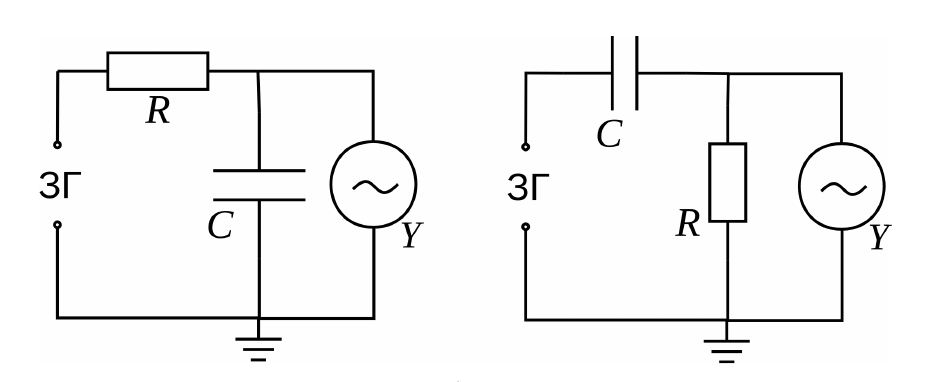
\includegraphics[width = 13cm]{7}}
	\caption{а) <<Интегрирующая>> ~б) <<Дифференцирующая>> цепочка}
	\label{fig:image}
\end{figure}

Сравним полученные зависимости с теоретическими:

$$K_a(f) = \frac{1}{\sqrt{(\omega t)^2 + 1}}$$
$$K_b(f) = \frac{1}{\sqrt{(\omega t)^{-2} + 1}}$$

\noindent где $\tau = RC$ --- постоянная времени RC-цепочки, $\omega = 2\pi f$ — циклическая
частота.







\end{document}

